%!TEX root = ../../Diplomarbeit.tex
\section{Case Study: Gamification in Plant Up!}
``Plant Up!'' \cite{plantUpProject} is a gamified smart gardening system that combines IoT sensors with a mobile application to provide users with an engaging way to monitor 
and care for their plants.
How does the gamification concept in ``Plant Up!'' \cite{plantUpProject} work in practice? 

\subsection{Evaluation and Discussion}
The core goal of integrating gamified mechanics into Plant Up! \cite{plantUpProject} is to bridge the gap between dry, technical plant monitoring and sustained, long-term user engagement. 

\subsubsection{Meaningful Habit Formation}
Examining core mechanics like XP, daily streaks, and the in-game ``XP Booster'' reveals that the system leverages classical behavioral psychology to foster sustainable habit formation. 
What distinguishes Plant Up! \cite{plantUpProject} is that these rewards are not arbitrary digital tasks. Because they are directly tied to real-time data from smart IoT sensors, the rewards are grounded in the actual biological needs of the plants. 
This creates a framework of meaningful gamification: by providing structured extrinsic rewards (XP and coins) during the slow biological latency phases (the waiting periods before visible plant growth occurs), the system bridges the motivation gap until the intrinsic reward, such as a healthy, blooming plant, is achieved. This effectively puts the core concepts of Self-Determination Theory (SDT) \cite{ukcoachingSDT} into practical application.

This smooth transition from extrinsic nudges to intrinsic satisfaction leads naturally into how the system supports beginners who have yet to develop those intrinsic connections.

\subsubsection{Lowering the Entry Barrier}
One of the primary strengths of the Plant Up! \cite{plantUpProject} approach is how effectively it lowers the barrier to entry for complete beginners. This is a significant structural advantage because it directly mitigates the steep learning curve often associated with botany, actively supporting the ``Competence'' pillar of SDT. 
Through ``Sprig,'' the friendly NPC guide, and a system of structured quests, the application translates complex botanical sensor data into simple, actionable feedback (see Figure \ref{fig:plantup_sprig_tutorial}). 

\begin{figure}[H]
    \centering
    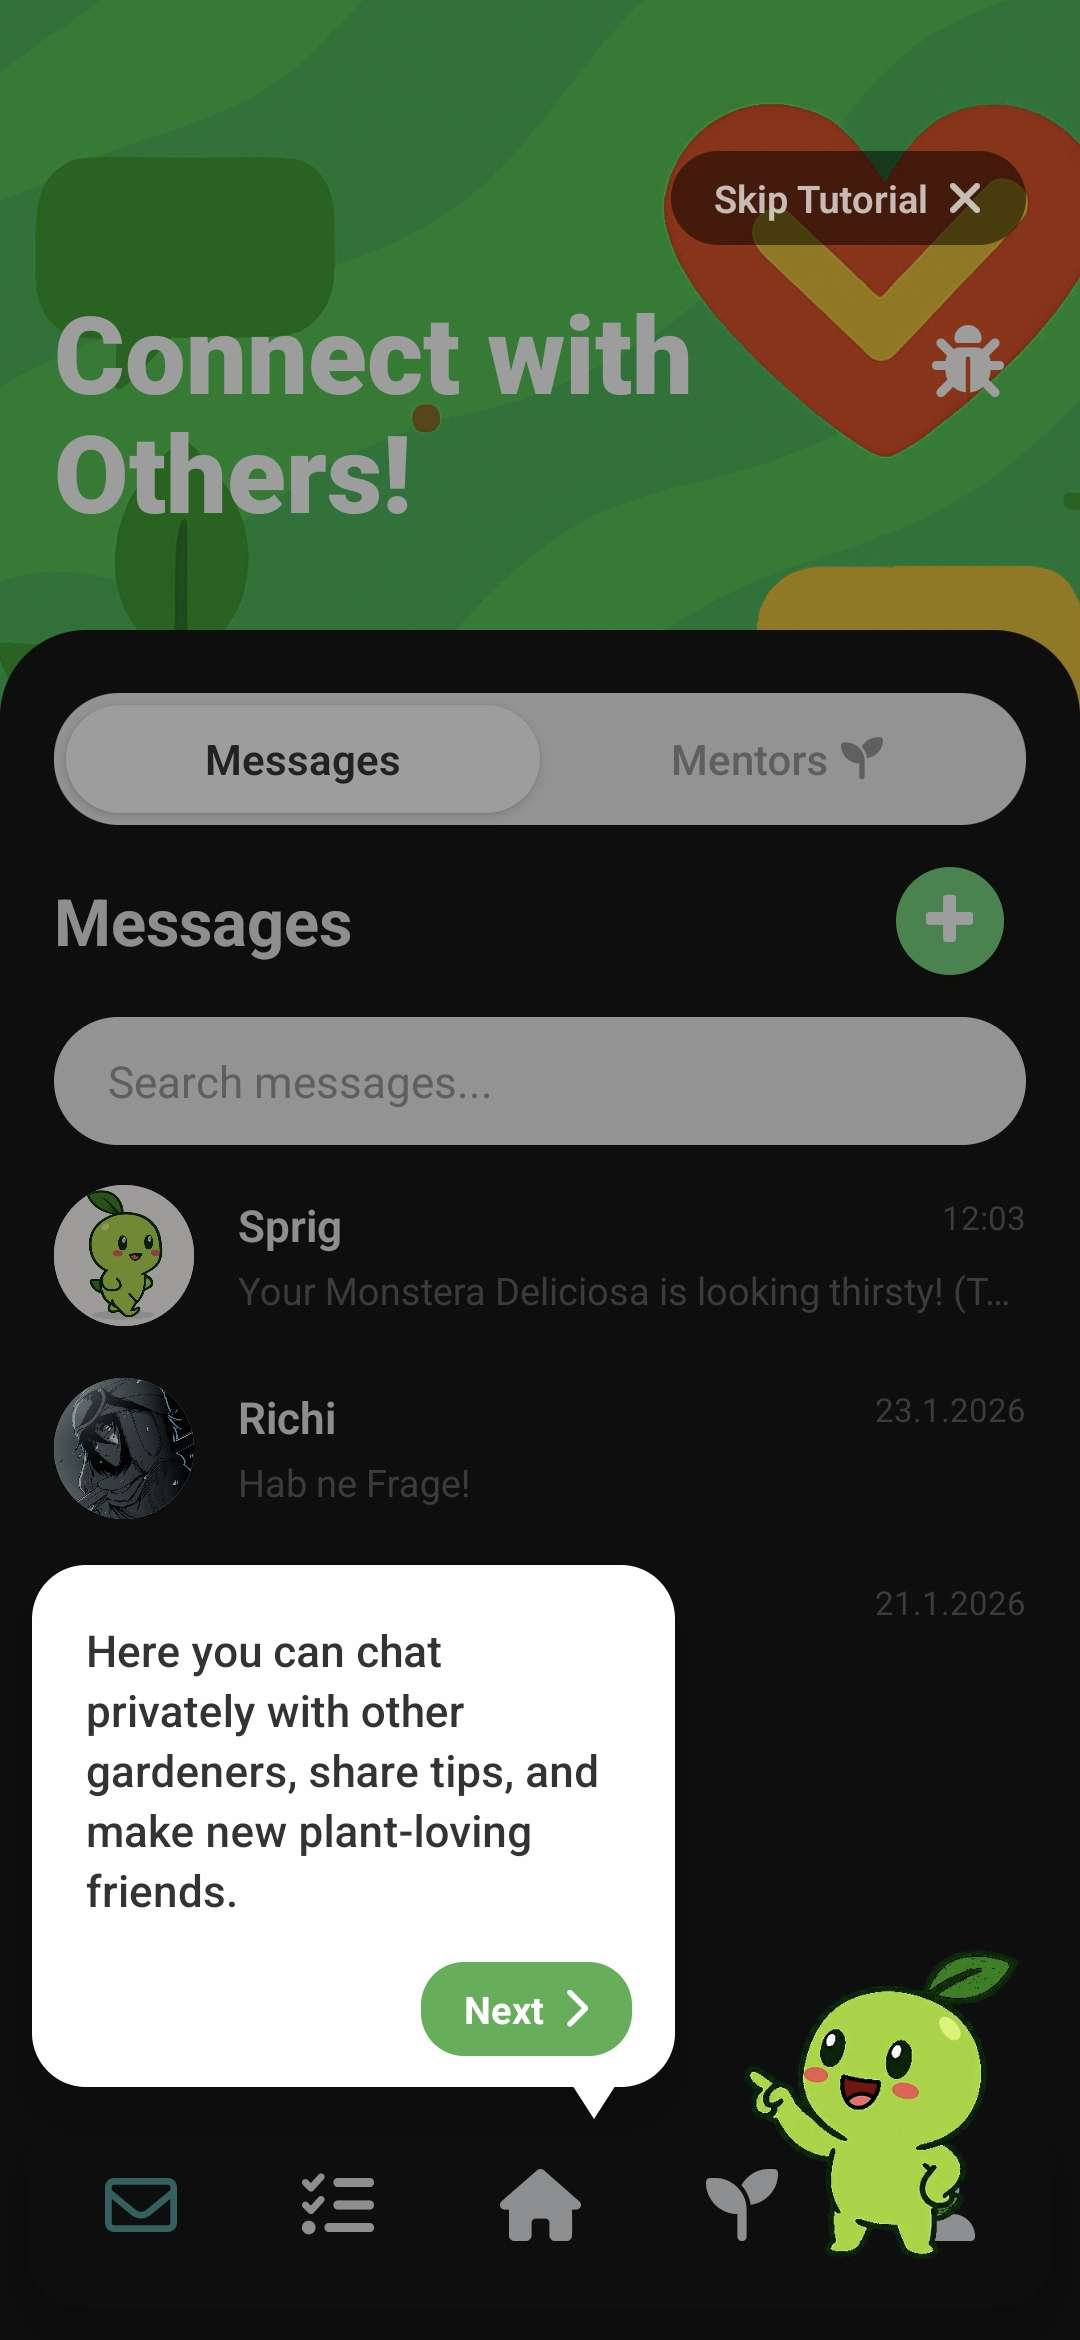
\includegraphics[width=0.45\textwidth]{images/sprig.png}
    \caption{The Plant Up! NPC guide ``Sprig'' providing tutorials and easily understandable feedback to help new users \cite{plantUpProject}.}
    \label{fig:plantup_sprig_tutorial}
\end{figure}

These elements directly address a common pain point in gardening: the feeling of being overwhelmed by plant care demands. 
Furthermore, items like the ``Freeze Streak'' and ``XP Boosters'' in the shop demonstrate a sophisticated understanding of long-term retention. 
These features actively mitigate loss aversion (the psychological tendency to feel losses more strongly than equivalent gains), which intensifies when a user inevitably misses a day of care. 
By offering a safety net, the system prevents the devastating loss of progress that typically causes users to abandon an app out of frustration.

While these mechanics effectively address beginner anxiety and build early engagement, they introduce a separate set of risks that must be managed as the user matures.

\subsubsection{Potential Long-Term Challenges}
Relying heavily on extrinsic motivators such as virtual coins and titles does present potential long-term challenges.
This represents a structural disadvantage because it can condition users to engage only when an external reward is present, rather than developing genuine, self-sustained interest in the activity \cite{ukcoachingSDT}. 
While these mechanics are effective for building initial habits, there is a risk of the ``over-justification effect'' (the phenomenon where excessive external rewards gradually erode a person's intrinsic interest in a task). 
Users may eventually start prioritizing digital rewards and leaderboards over the actual health of their physical plants. 
If the gamification layer becomes too dominant, the primary utility of the IoT sensor data, ensuring plant survival, could be overshadowed by the pursuit of online status. 
Additionally, designers must guard against ``statistical anxiety,'' the stress that can arise from public social features when users feel intense pressure to maintain perfect streaks. This risks turning what should be a relaxing hobby into a source of digital stress \cite{plantUpProject}.

To counteract these effects, the system relies on communal features that foster the ``Relatedness'' aspect of SDT, requiring a robust technological foundation.

\subsubsection{Technical Architecture \& Community}
From a technical perspective, the architecture of Plant Up! \cite{plantUpProject} efficiently handles the constant stream of sensor data and user-generated content, such as shared plant-care videos and social posts, by utilizing an ASP.NET API coupled with Supabase. 
This social dimension is crucial for long-term viability because it elevates the app from a solo monitoring tool into a knowledge-sharing community, thereby fulfilling the human need for social connection and actively supporting the third pillar of SDT (Relatedness).

Looking ahead, future technical enhancements will likely need to focus on Android animation normalization. 
Ensuring that the gamification UI remains fluid across a wide variety of mobile hardware is essential, as any technical friction or lag in the animations can instantly break the ``flow'' state (the mental state of complete, effortless immersion in an activity) required for an engaging user experience \cite{plantUpProject}.
